\documentclass[11pt,a4paper]{article}
\usepackage{od,wrapfig}
\usepackage[utf8]{inputenc}
\usepackage[main=english,russian]{babel}
\usepackage{tikz}
\usetikzlibrary{shapes.misc, arrows.meta}
\usetikzlibrary{arrows, decorations.markings}

\newcommand{\bbox}[2]{\parbox{#1cm}{\small\centering #2}}

\tikzstyle{vecArrow} = [thick,
  decoration={markings,mark=at position 1 with {
      \arrow[semithick]{open triangle 60}
    }
  },
  double distance=1.4pt, shorten >= 5.5pt,
  preaction = {decorate},
  postaction = {draw,line width=1.4pt, white,shorten >= 4.5pt}
]

\title{Human and Technical System} 

\author{Nikolay Shpakovsky, Minsk}

\date{January 20, 2003}

\begin{document}
\maketitle

\begin{quote}
  The original Russian text consists of two parts, which are combined here.
  
  Part 1: \url{http://www.gnrtr.ru/Generator.html?pi=201&cp=3}\\
  Part 2: \url{http://www.gnrtr.ru/Generator.html?pi=200&cp=3}
\end{quote}

\section*{Is a human a part of a Technical System or not?}
\begin{flushleft}
  ... the last words of the book of the prophet Lustrog read: «all true
  believers break eggs from whichever end is more convenient».\\
  Jonathan Swift «Gulliver's Travels»
\end{flushleft}

\section*{Introduction}
The Theory of Inventive Problem Solving (TRIZ), developed by the talented
engineer, inventor and ingenious thinker G.S. Altshuller, is widely known and,
undoubtedly, the most effective tool for solving engineering problems at
present time. A large number of materials have been published in Russian and
English languages, in which the essence of the theory is quite fully revealed
for an initial acquaintance with her. The best Russian-language resource is
the Minsk website center OTSM-TRIZ\footnote{\url{http://www.trizminsk.org}},
the best English-speaking is the American TRIZ
Journal\footnote{\url{http://www.triz-journal.com}}. Having studied TRIZ from
books and articles, you can easily teach others -- the material is so rich and
fascinating that interest in the classes will be ensured.

However, for a deeper understanding of TRIZ, one has to think through the
material, first of all, of the concepts and terms of TRIZ. This is required,
since most of the TRIZ material is presented for further reflection, and not
set up for simple memorization.

During my work for SAMSUNG as a TRIZ consultant, I had anew and seriously to
rethink everything that I knew about TRIZ before. When solving technical
tasks, bypassing patents of competing companies and developing a development
forecast of technical systems, it was very important to understand the deep
content of each TRIZ term in order to use its tools with maximum efficiency.

One of the basic concepts in TRIZ and one of the most important links to all,
without exception, of its tools is the concept of a «Technical System». This
term is introduced in classical TRIZ without definition, as a derivative of
the concept of a «System». But with closer examination, it becomes clear that
this concept «Technical System» requires further specification. This statement
is supported, for example, by semantic aspects.  The concept of «Technical
System» is translated from Russian into English in two ways: «Technical
System» and «Engineering System». Using any search engine on the Internet, it
is easy to convince yourself that these concepts are practically equal for
TRIZ specialists. Or take, for example, the glossary of Victor
Fey\footnote{\url{http://www.triz-journal.com/archives/2001/03/a/index.htm}},
in which there is simply no explanation of either one or the other concepts.

In this article, I tried to describe my understanding of the term «Technical
System», gradually developed after the solution of a specific problem, which
challenged me to find out the full composition of a minimum operational
technical system.

\section*{An attempt to analyze the concept «Technical System»}

First, let's consider what a general system is. There are many different
definitions of a system. The most dashing, abstract, therefore absolutely
exhaustive, but with little use for practical purposes was given by
B.R. Gaines [1]: \textbf{«The system is what we define as a system»}. In
practice, the most often used definition of a system is due to A. Bogdanov
[2]: \textbf{«A system is a set of interconnected elements with a common
  (systemic) property that is not reducible to the properties of these
  elements»}.

What is a «Technical System»?

Unfortunately, G. Altshuller did not dierectly define the concept of a
«Technical System». It is clear from the context that this is some kind of
system related to technology, to technical objects. As indirect definition of
a Technical System (TS) can serve the three laws formulated by him, or rather,
three conditions that should be satisfied for its existence [3]:
\begin{itemize}[noitemsep]
\item[1.] The law of completeness of the parts of a system.
\item[2.] The law of «energy conductivity» of the system.
\item[3.] The law of harmonization of the rhythms of the parts of the system.
\end{itemize}
According to the law of completeness of the parts of a system, each TS
includes at least four parts: engine, transmission, working body and control
system.  
\begin{center}
\begin{tikzpicture}[
    >={Triangle[length=3pt 9, width=3pt 3]},
    rounded corners=2pt]

  \draw[fill=yellow] (1.2,1.5) -- (8.8,1.5) -- (8.8,4.5) -- (1.2,4.5) --
  (1.2,1.5) ;

  \node[draw] at (5,3.5) [rectangle] (A0) {\bbox{2}{Control System}};
  \node[draw] at (2.5,2) [rectangle] (A1) {\bbox{2}{Engine}};
  \node[draw] at (5,2) [rectangle] (A2) {\bbox{2}{Transmission}};
  \node[draw] at (7.5,2) [rectangle] (A3) {\bbox{2}{Working Organ}};
  \node[draw] at (12,2) [rectangle] {\bbox{2}{Processed Object}}; 
  \draw (0,2.5) node {\bbox{2}{Energy Resources}}; 
  \draw (9.7,2.3) node {{\small Action}}; 
  \draw[->] (A0) -| (A1) ;
  \draw[->] (A0) -- (A2) ;
  \draw[->] (A0) -| (A3) ;
  \draw[vecArrow] (-1,2) -- (1,2) ; 
  \draw[vecArrow] (8.9,2) -- (10.7,2) ; 
\end{tikzpicture}\\
Minimal structure of a technical system capable to work according to
G. Altshuller.
\end{center}
That is, there is some kind of system, a machine consisting of technical
objects, subsystems that can perform the required function. It includes a
working body, transmission and engine. Everything governing the action of this
machine is placed in the «control system» or a not well understood «cybernetic
part» [4].

The important thing here is the understanding that the TS is created to
perform some function. Probably, this should be understood in such a way that
a minimally TS capable to work can perform this function at any time, without
additional supplementation. Ways to the definition of a Technical System are
given in the book «Search for New Ideas» [5], where the definition of a
«Developing Technical System» is given. This question is touched by V. Korolev
in his interesting studies [6,7]. Some critical remarks are devoted to this
topic also in the materials of N. Matvienko [8]. The definition of the concept
of a «Technical System» in relation to TRIZ is given by Yu. Salamatov in [9]:
\begin{quote}\bf
  A Technical System is a set of orderly interacting elements, which has
  properties that can not reduced to properties of individual elements and
  intended to perform certain useful functions.
\end{quote}
Indeed, a human has some kind of needs, for the satisfaction of which it is
necessary to perform some function. Hence you need somehow to organize a
system, performing this function -- the Technical System -- and satisfy the
need.

What is confusing in the above definition of a Technical System? The word
«intended» is not quite clear. Probably, it's not someone's wishes that are
important here, but the objective ability to perform the required function.
\begin{quote}\it
  For example, what is a metal cylinder for with an axial hole with variable
  diameter and threaded at one end?

  It is almost impossible to answer such a question. The discussion is
  immediately switching to the level of the question «where it could be
  applied?».
\end{quote}
But is it possible, using this definition, to say: Until now this is not yet a
Technical System, and from now on -- it is? It is written like this: «... the
TS appears, as soon as the technical object acquires the ability to perform
the Main Useful Function without a human.» And then it is claimed that one of
the trends in the development of the TS is the removal of the human from its
parts.  This means that at some stage of TS development, a human is part of
it.  Or not? Unclear ...
\begin{quote}\it
  We probably won't understand anything if we don't find an answer to the
  question: is the human part of a Technical System or not?
\end{quote}
Having interviewed several TRIZ experts, I received a fairly wide range of
answers: from a firm «No», backed up by references to big experts, to a timid
«yes, probably».

The most original of the answers: when the car moves evenly and straight 
-- the human is not part of this technical system, but once a car begins to
turn, then the human immediately becomes a necessary and useful part of it.

What's in our literature? Salamatov [9, Section 4.3] gives an example that a
man with a hoe is not a TS. Moreover, the hoe itself is not a Technical
System.  But a bow is a TS.

But what is the difference between a hoe and a bow? The bow has an energy
accumulator -- string and flexible rod, in a good hoe, too, when swinging, the
handle bends and when moving down increases the force of the blow. It bends a
little, but it's about the principle. The bow work in two movements: first it
is cocked, then released, with the hoe -- too. Why then such an injustice?

Let's try to figure it out.

A sharpened wooden stick is a Technical System? Does not look like it. And an
automatic pen? This is probably a TS, and a quite complex one. And what about
a printer? Undoubtedly TS.

And a pencil? Who knows ... It seems like neither this nor that. Maybe call it
«simple Technical System»?  Lead or silver writing stick? Question ...
Already not a splinter of wood, after all -- a precious metal, but it is
still far from the pen.

A modern capillary pen, a pencil, a sharpened stick and the writing unit of a
printer -- what do they have in common? Some useful function that they, in
principle, could perform: «leave a mark on the surface».

«Lanky Timoshka is running along a narrow path. His traces is your labor».  Do
you remember?  This is a pencil. And also a stick, lead or silver stylus, pen,
felt-tip pen, printer, printing press. What a set! And the row is logical ...

However, here again a question arises.

If all these objects can perform the same function, then they all are
Technical Systems. And there is no need to divide them into complex and
primitive ones. If objects implement the same functions, then they have not
only the same purpose, but also the level of hierarchy should be the same.

Or vice versa -- these are all not TS. Well, what a Technical System -- a
sharpened stick? Where is its engine or transmission? But then it turns out
that the printer is also not a TS.

Let's be formal.

Any Technical System must perform some useful function. Can the sharpened
stick fulfill its function? No. And the printer?

Let's do a simple experiment. Place the pen on the table. Or, for simplicity,
on the paper. Let’s just wait until it begins to perform its main useful
function.  Does not. And it will not perform until a human, the operator,
takes it in his hand, does attach it to a sheet of paper, and «... the verses
will flow freely».

And the printer? Will he start typing until the user gives a command to the
computer, and this one in its turn, does forward it to the printer? That is,
without pressing a button, a voice or, in perspective, a mental command, the
action will not happen.

Thus, the following is obtained. A pen, a hoe, a printer, a bicycle are not
TS.  More precisely, not complete TS. They are simply «systems of technical
objects». Without a human, an operator, they cannot work, i.e. cannot fulfill
their function. Of course, in principle -- can, but in reality ... In the same
way, four wheels, a body and a hood can't nothing transport ... Even a fully
equipped brand new car, refueled lonely, with key in the ignition lock, is not
a Technical System, but simply a «system of technical objects». If the
operator will sit down on his place, in common language, the driver, takes
rushes behind the wheel, and immediately the car becomes a Technical System.
And all others technical objects and systems become complete TS and operate
only and exclusively together with a human, the operator.

The operator can sit inside the «system of technical objects». Can stand near
it, farther or closer. Can even program the action of the Technical System,
turn it on and leave. But in any case -- the operator must participate in the
TS management.

And no reason to oppose the spaceship and the hoe. Both the first and the
second -- this is a greater or lesser part of a certain TS, which for normal
execution of the main useful function must be supplemented with one or more
operators.

Let us recall the law of completeness of the parts of a system, formulated by
G.S. Altshuller. A TS arises when all four parts are present (Fig. 1), and
each of them should be minimally capable to work. If at least one part is
missing, then this is not a Technical System. It is also not a TS if one of
the four parts is not working. It turns out that the Technical System is
something that should be completely ready for immediate fulfillment of its
main useful function without additional completing. Like a ship that is ready
to cast off.  Everything is filled up, charged up and the entire crew on their
places.

And without human, the control system is not only not «minimally capable to
work», but not capable to work in principle, since it is not staffed. The law
of completeness of the parts of the system is not fulfilled. And the law of
energy conductivity is not fulfilled. There is a signal going into the control
system, and -- stop. There is no reverse flow of energy.

And what about those «Technical Systems» that successfully perform their
useful function, but do not contain technical objects at all? For example,
the electrician changing a light bulb ...

It seems that there is such a special level of the hierarchy at which a
collection of objects, elements turns into an actual Technical System. This is
the level of a car with a driver, a video camera with operator, a pen with a
writer, an automated production in a water complex with operators who start
and maintain it, etc.  This is the level at which the system is formed: a set
of natural and technical objects, a human operator and his actions, who is
performing some kind of a directly useful for humans function.

It is interesting to see how the hierarchy of biological objects and systems
is built. Molecules, cells, elements, parts of organisms -- this are the
levels of subsystems.  A «Subsystem» is a separate part of a body, for
example, the skeleton of an elephant, the sting of a mosquito or a feather of
a titmouse.  The sum of such subsystems, even their complete set, an organism
entirely assembled from them, cannot perform useful functions. You need to add
something else to this «set», breathe in a «spark of God» to get a living,
functioning organism.
\begin{center}
 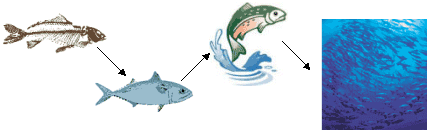
\includegraphics[width=.6\textwidth]{mts-2.png}
\end{center}
Living organisms, individuals, can be combined into a supersystem.  A
«supersystem» is more or a less an organized collection of animals or plants,
such as a bee family.  But such a sharp qualitative leap does not occur here.

By analogy with biological systems, the concept of a «Technical System» can be
considered as a special level of the hierarchy, at which the system gets the
opportunity to act independently, i.e. at the level of a living organism.

In other words, the «Technical System» in technology corresponds to the level
of a living organism in nature. In a patent application, this is called
"machine in operation". That is, «the system of technical objects» plus a
human operator. For example, a carburetor is not a TS, but simply a system, a
set of technical objects. But the human (operator), knocking with the
carburetor on a nut is a TS with a useful function: to peel nuts from the
shell.  So a man with a hoe is a TS, but a tractor with a plow is not.
Paradox ...

\begin{quote}\it
  «Human» -- what is this applied to a Technical System?  What is here
  difficult for understanding?
\end{quote}
The confusion is probably caused by the very wording of the question.  It is
psychologically difficult to put a human and a shoe brake on the same level.

There is no doubt that human, as part of the technosphere, has the most direct
relation to any TS and can be in relation to it in the following role
situations:

\emph{In the supersystem:}
\begin{itemize}[noitemsep]
\item[1.] As user.
\item[2.] As developer.
\item[3.] As manufacturer of the technical objects of the system.
\item[4.] As person providing maintenance, repair and disposal of equipment
  system objects.
\end{itemize}
\emph{In the system:}
\begin{itemize}[noitemsep]
\item[1.] As operator, the main element of the control system.
\item[2.] As source of energy.
\item[3.] As engine.
\item[4.] As transmission.
\item[5.] As working body.
\item[6.] As the processed object.
\end{itemize}
\emph{In the environment:}
\begin{itemize}[noitemsep]
\item[1.] As element of the environment.
\end{itemize}
The user is undoubtedly the main person. It is he who pays for the creation of
the TS, at his will, developers and manufacturers get down to business. He
pays for the operator's labor, maintenance, repair and disposal of technical
objects of the system.

The second group of persons ensures the functioning of the TS during work,
feels its impact on itself.

The third group indirectly helps or hinders this process, or simply observes
gives behind it and is exposed to the side effects that occur during
operation. 

A person can fulfill several roles at the same time. For example, the driver
owning the car or a person using an inhaler. Or a bicyclist. He is an element
of almost all bicycle subsystems, except for the working body (seat) and
transmission (wheels and bike frame).

\emph{Still, it turns out that a human is an obligatory part of the Technical
  System}.

It seems what does it matter. After all, how it comes down to it, to the
solution of real engineering tasks, then human quickly leaves the problem zone
and has to work at the level of subsystems. Yes, but only in those places
where the coordination and passage of energy is carried out between subsystems
not connected in any way with the operator. But if we come closer to the
control system the problem of human interaction with technical objects grows
up in full size.

Take a car, for example. The car acquired its current appearance by the end of
the 1970s, when airbags and a reliable automatic transmission were invented.
Most of the improvements since then are aimed only to improve management,
safety, ease of maintenance and repair, i.e., on the interaction of a human,
the main part of the TS, with its other parts.

The truck of the 1940-50s had a steering wheel with a diameter of 80 cm. The
driver must be very strong to drive such a car. And in aviation ... the giant
airplane of the 1930s «Maxim Gorky». To perform a maneuver, at the contol
stick the first and second pilot had to pull together. Sometimes they called
the navigator for help and the rest of the crew. Nowadays the operator with
the help of amplifiers can control much more loaded mechanisms. It seems the
problem has been solved. But no, again often the human is forgotten ... The
fact is that amplifiers do not always allow the operator to fully feel the
behavior of the controlled mechanism. This sometimes leads to accidents.

For example, the problem of the safety of driving a car or the more
«monotonous» locomotive management. It is very important that the operator is
always in an alert, workable state. This problem is also solved in the
supersystem -- causes we fall asleep while driving are removed, medical
control is carried out, the responsibility of the driver-operator is
increased.  But increasingly it is solved directly in the Technical System.
Right in the cabin. If the driver does not turn off the warning light in time,
the engine is stopped and the train slows down. Or in a car: you won't go
until you fasten your seatbelt.  That is, there is a normal feedback in the
same way as between all other elements of the TS.

Perhaps one of the reasons why this direction of improving technical systems
began actively to develop actively in recent years is a lack of understanding
of the place of human in their structure. Rather, not that not understanding,
but ... In general, the developer finds himself in a difficult psychological
situation. As human the developer of something new rightfully feels like a
creator. He cannot fully feel that a human can also be an operator, engine or
working body, a part of the mechanism, the machine, the Technical System.
It's good yet if it's a widely used TS that closely interacts with a human,
for example, a car. Here a person can be a developer, an operator and a user
at the same time.

As with a computer. It is difficult to work with most computer programs even
today, when the developers understood the simple truth, that with the program
will work a human operator who cares about the result, not the construction of
the device. Today such concepts as «user friendly interface» were introduced.
But earlier ... Why walk far, remember «Lexicon».

And other TS, standing, at first glance, far from the human ... Their name is
legion. Here often the thought does not even occur that human is a part of the
Technical System.  But when developing any of them, it is necessary to analyze
the interaction of the elements composing the system and taking into account
the capabilities of the human body and mind. Sometimes it is not done.

Even worse, often many of the known natural factors are not taken into
account, affecting the well-being of humans, the clarity of their movements
and the speed of reaction. A newly discovered psychological factors, for
example, the «Cassandra effect» [10]?

It rises Chernobyl as terrible mushroom, airliners fall and ships collide.

\emph{But what else, besides the operator, is needed to get a ready-to-operate
  Technical System?}

\section*{The complete composition of a minimally capable to work Technical
  System} 

There is a set of technical objects combined into a system, there is a human
operator. Is this enough for the Technical System to perform a useful function
and to satisfy user's need, or do you need something else?

Let us recall the well-known TRIZ example given in the book by G. Ivanov [11].
We are talking about the Russian scientist Kapitsa, who visited the Simmens
and Schuckert plant on production of generators. The owners of the plant
showed him the generator, which did not want to work and offered 1000 marks
for correction. Kapitsa quickly realized that the central bearing was skewed
and jammed, took a hammer and hit the bearing housing -- the generator started
working.  The confused customers asked for an invoice for the work performed.
Kapitsa wrote: \emph{«1 blow with a hammer -- 1 mark, for knowing where to hit
  -- 999 marks»}.

And here is another example from Fenimore Cooper [12].

The heroes of the story run away from the chase, the Indians drove them into
thickets of tall dry grass and set it on fire. The fire goes like a wall, what
to do? The old hunter was not taken aback and set fire to grass near where
they stood. The wall of fire went towards the one who overtook them fiery
shaft, burning fuel for it. The fire went out, those who fled escaped.

What is a Technical System in the one and the other case?

In the first example. The user's need is to start the generator. Useful
function -- align the bearing. Operator -- Kapitsa, system of technical
objects -- hammer.  It turns out that the Technical System is Kapitsa with a
hammer.

In the second example. The user's need is to stop the fire. Useful function --
destroy the grass (fuel for the coming fire). The operator is an old hunter,
the system of technical objects -- flint and steel.

Technical System -- a hunter with flint and tinder.

What's coming out? A minor action of a human operator using a primitive
technical means gave such a tremendous result both in the first and second
case! Is that all? Is it really a complete set of technical systems, action
which allowed in the first case to start a huge generator, and in the second
-- to stop a wall of fire?

No, it’s not.

The most important thing is that which was completely overlooked in the
previous reasoning -- informational component.

Indeed, you can uselessly hammer on the generator from morning to night. But
Kapitsa knocked not at random, but in a strictly defined manner. And in this
case, the informational support of his actions consisted of two parts: «the
ability to knock with a hammer» and the knowledge, understanding of «where to
hit».

In the same way, setting fire to the grass could be completely useless, and
most of the variants could end in disaster for the one who set it on fire.

If we further analyze the second example, it becomes obvious that the burning
dry grass makes sense when the hunter not only knows that the wind can drive
the fire towards the approaching fire, but if the wind blowing in the right
side is present.

Therefore, it is very important to know «how to do it?», how to perform a
useful function, using for this technical objects and available
substance-field resources that also become part of the TS during its
operation.

To complete a full minimum capable to work TS, it is necessary to take
into account the following informational and material components:
\begin{itemize}[noitemsep]
\item[1.] The technological process of performing the useful function.
\item[2.] Material technical and natural objects and systems of different
  levels of hierarchy.
\item[3.] One or more operators who own a set of control techniques of the
  material objects and systems.
\item[4.] Substances and fields necessary for the operation of the material
  objects and systems, and the products of their processing.
\item[5.] Substances and fields necessary for the functioning of the operator,
  and the products of their processing.
\item[6.] The processed object (in some cases).  
\end{itemize}
Full composition of a Technical System:
\begin{center}
\begin{tikzpicture}[rounded corners=2pt] 
  \draw[dashed,rounded corners=6pt,fill=gray!10] (7,1) -- (7,-1) -- (13,-1) --
  (13,1) ; 
  \draw[dashed,rounded corners=20pt,fill=gray!20] (2,5.25) -- (2,1) --
  (17,1) -- (17,5.25) ; 
  \draw[dashed,rounded corners=20pt,fill=yellow!30] (2,5.25) -- (2,7.5) --
  (17,7.5) -- (17,5.25) ; 

  \node[draw=green] at (5.5,6.5) [rectangle] (A0) {\bbox{6}{Information about
      the realisation of the technical process}}; 
  \node[draw=green] at (13.5,6.5) [rectangle] (A1) {\bbox{6}{Knowledge how to
      work with the system of technical objects}}; 
  \node[draw=red] at (5,4) [rectangle] (A2) {\bbox{5}{Systems, objects,
      substances and fields for the operator's actions}}; 
  \node[draw=red] at (5,2) [rectangle] (A3) {\bbox{5}{Systems, objects,
      substances and fields for the actions of the system of technical
      objects}}; 
  \node[draw=blue] at (14,4) [rectangle] (A4) {\bbox{3}{Processing products}}; 
  \node[draw=blue] at (14,2) [rectangle] (A5) {\bbox{3}{Processing products}}; 
  \node[draw=blue, line width=2pt] at (10,4) [rectangle] (A6)
       {\bbox{2}{Operator}}; 
  \node[draw=blue, line width=2pt] at (10,2) [rectangle] (A7) {\bbox{2}{System
      of technical objects}}; 
  \node[draw,fill=blue!30] at (10,0) [rectangle] (A8) {\bbox{4}{Processed
      object}}; 
  
  \draw[color=red] (15,5.6) node {\small Level of information};
  \draw[color=red] (15,4.9) node {\small Object level};
  
  \draw[->] (A0) -- (A6) ;
  \draw[->] (A1) -- (A6) ;
  \draw[->] (A2) -- (A6) ;
  \draw[->] (A6) -- (A4) ;
  \draw[->] (A3) -- (A7) ;
  \draw[->] (A7) -- (A5) ;
  \draw[vecArrow] (A6) -- (A7) ; 
  \draw[vecArrow] (A7) -- (A8) ;
\end{tikzpicture}
\end{center}
It is in this composition that the TS gets the opportunity to work everywhere,
in any place and full autonomy.  Even in zero gravity and airless space.

This approach -- complete a TS with everything necessary to carry out its
useful features -- does not override the traditional one, but is quite
convenient. Collect everything you need to perform the function into one
system and transform it, mentally separating it from the supersystems. It is
easier to do any job if you prepare in advance all the necessary materials,
tools and drawings, arrange it in the most convenient way not to rummage later
on around the "workshop" (supersystem), remembering what else is required to
provide ensuring the capability of our TS to work.

That is, the Technical System is the supersystem for the System of technical
(material) objects.

This understanding of the TS has something in common with its description
given by N. Matvienko [8]: \textbf{«Every Technical System is a set of
  material, energetic and information elements (in other words, real parts and
  details, energy resources for their functioning and a set of prescriptions,
  instructions, commands, signals that determine the sequence and type of
  interactions of material elements with surrounding systems and with each
  other)»}.

This approach puts the human operator at the center, in the basis of the
Technical System.

At the same time, a "Technical System", organized by a human, may include the
use of object like technical or natural elements -- for example, acupuncture
or transportation of goods, as well as avoiding them altogether -- the speech
of a lawyer in the court or a dance. This sometimes changes little. As example
of this statement may serve a lawyer speaking to the audience with or without
a microphone.

But, if you really look at it, then a human is a multifunctional Technical
System, too.  Human nature is twofold -- he has the ability to think, to model
his actions, to make decisions. And act using his body to do some work.  It is
here where the informational and material components of a human unite into a
single entity.

The human operator includes all the main parts of a TS and, subject to
information and material support, can perform some functions, in accordance
with the possibilities of his body. When these possibilities are exhausted,
one can add to the body material objects, combine them into systems and expand
the capabilities of the human. The normal process of enfolding a Technical
System begins. A rock, stick, shovel, excavator ... Human is getting stronger,
he can fulfill a more and more increasing amount of work.

And what about folding?  After all, it seems that it is already impossible to
fold a human. Yes, when talking about folding objects. But here the folding is
on the information level.

For example, it's time to water the garden. One can take a water can, adapt a
water tube, set up a whole irrigation machine. Or you can just look at the sky
and, if it is raining soon, you don't have to do anything. That is, folding
occurs at the level of functions, technological operations. Finally, at the
level of systems and process design. TRIZ itself is a logical continuation of
this direction. After all, the concepts of «Ideality», «Ideal Final Result»
are basic concepts of this methodology.

This was noticed a long time ago, and a rare fairy tale avoids a part where
something is going on by itself, a person achieved what he wanted without any
expenses.  The power of thought, so to say, breaks mountains. Move in time and
space. A «technical task» on human development in this direction are
prescribed by science fiction writers and storytellers.  And there are reasons
to think that this direction will be mastered. Levitation, moving objects with
glances, communication over long distances without any technical means and
much more -- all this can be accessible to humans.

Yes, this is interesting, but what does all of the above give for
transforming, improving Technical Systems in real practice?

\textbf{A dramatic increase in the amount of resources that can be acquired
  for change when transforming the system.}

\emph{In the traditional approach the following resources can be used:}
\begin{itemize}[noitemsep]
\item[1.] The system itself.
\item[2.] Its subsystems.  
\item[3.] Connections between subsystems.
\item[4.] Links between each subsystem and
system.  
\end{itemize}
\emph{With the proposed approach, the number of possible resources for use
  increases dramatically. Here are just a few of them:}
\begin{itemize}[noitemsep]
\item[1.] The Technical System itself.
\item[2.] The Technological process.
\item[3.] Technological operations.
\item[4.] The System of technical objects.
\item[5.] Subsystems of the system of technical objects.
\item[6.] The operator as a thinking system.
\item[7.] The body of the operator, as a material biological system.
\item[8.] Sense organs of the operator.
\item[9.] The system of skills of the operator.
\item[10.] Individual skills of the operator.
\item[11.] Systems, objects, substances and fields consumed by a system of
  technical objects.
\item[12.] Systems, objects, substances and fields consumed by the operator.
\item[13.] Relations between the Technical System and the technological
  process.
\item[14.] Relationships between technological operations and the
  technological process.
\item[15.] Relationships between technological operations.
\item[16.] Relations between the Technical System and technological
  operations.
\item[17.] Interaction of substances and fields consumed by the Technical
  System with a system of technical objects.
\item[18.] Interaction of substances and fields consumed by the Technical
  System with the operator.
\item[19.] Connections between subsystems of the system of technical objects.
\item[20.] Connections between each subsystem of the System of Material
  Objects and the system of technical objects.
\item[21.] Relationships between the subsystems of the system of technical
  objects and the technological process.
\end{itemize}
... And many other combinations of elements of the Technical System ...

It's time to give some examples.

%-------------------

\paragraph{1. Classic airplane.}
A classic airplane of the beginning of the twentieth century consists of two
wings that were attached to the fuselage with the help of numerous struts and
cable guides. To make such a plane well flew (this was especially important
for air fighters), the stretched cables must be properly tensioned. Since the
cables under tension are further stretching they often had to be adjusted
using a simple screw mechanism. They applied a special ruler, and the cable
was pulled with a dynamometer. About the degree of tensions they judged by the
deviation of the cable from a straight line. This process was very laborious
and slow.

How to be? How to speed up the process of adjusting the stretching?

Basically, a new system had to be invented to adjust the stretch marks. If
those who solved this problem would only start from the System of Material
Objects, used to perform this function, it would be extremely difficult to
solve it. If remember and take into account that there is an operator in the
system, then the number of possible conversions increases significantly. So,
you can solve the problem using the organs of sense of the operator.

Indeed, why not use hearing, or rather people with perfect pitch? Piano tuners
were invited to adjust the stretch marks, the adjustment process was
accelerated many times.

Interestingly, since there were not enough piano tuners, the next solution was
found, which demonstrates the repeatedly described TRIZ tendency «displacement
of human from the TS». Stretch adjustment was handed over to the mechanics
again, but instead of a bulky ruler and dynamometer it was suggested to use a
suitably configured tuning fork.

\paragraph{2. Oil lamp.}
It's hard to imagine what a titanic job was done by inventors who tried to
make an oil lamp shine well. All the problem was poor oil flow to the wick
tip. To improve the supply numerous spring based devices were created to build
up pressure in the oil reservoir. Pumps for forced oil supply were also used.
That is, work went within the framework of the «system of technical objects»
-- they tried to improve the machine. And when examined the full composition
of the TS, it became clear that the issue was not in the lamp device, but in
the combustible material. When instead of oil that was poorly absorbed by the
wick oil liquid kerosene was used, all problems disappeared.

\paragraph{3. Computer.}
Suppose you want to use your computer in the dark. If we transform the System
of Material Objects, then ideas about glowing keys, light bulbs and more come
to the thought. If you think about the Technical System, then the answer is
obvious -- the operator must be able to type in the dark, remember the
location of the keys by heart.

What can be said in conclusion? Now in TRIZ and other innovative methods the
concept of a «Technical System» is completely confused mixing up constantly a
system that \textbf{performs} some function, and a «System of technical
(material) objects», that is \textbf{designed} to perform some function.
Interfering as little as possible into the dispute between "sharp-edged" and
"blunt-edged" (see the epigraph), I tried to understand this matter.

Without calling the reader to agree with me, I will be glad if this attempt of
analysis turns out to be useful to him to some extent.

I am very grateful to colleagues V. Lenyashin, G. Severinets, E. Novitskaya,
N. Khomenko and to the merciless critic of the first version of this article
by V. Sibiryakov for his help in preparing this material.

\section*{Literatur}
\begin{itemize}
\item[1.] B.R. Gaines. General System research: Quo vadis? General System.
  Yearboor, 24, 1979.
\item[2.] A.A. Bogdanov. \foreignlanguage{russian}{Всеобщая организационная
  наука. Тектология} (General Management Science. Tectology). Book 1.  Moscow
  1989.
\item[3.] G.S. Altshuller. \foreignlanguage{russian}{Творчество как точная
  наука} (Creativity as an exact science).
  \url{http://www.trizminsk.org/r/4117.htm#05}.
\item[4.] A.F. Kamenyev. \foreignlanguage{russian}{Технические
  Системы. Закономерности развития} (Technical Systems. Development Patterns).
  Leningrad, Mashinostroenie 1985.
\item[5.] G. Altshuller, B. Zlotin, A. Zusman, V. Filatov.
  \foreignlanguage{russian}{Поиск новых идей: от озарения к технологии} (The
  search for new ideas: from insight to technology). Chisinau, Carta
  Moldaveniasca, 1989. S. 365.
\item[6.] V. Korolev. \foreignlanguage{russian}{О понятии «система»} (About
  the «system» notion). TRIZ Encyclopaedia.
  \url{http://triz.port5.com/data/w24.html}.
\item[7.] V. Korolev. \foreignlanguage{russian}{О понятии «система»} (About
  the «system» notion) (2).  TRIZ Encyclopaedia.
  \url{http://triz.port5.com/data/w108.html}.
\item[8.] N.N. Matvienko. \foreignlanguage{russian}{Термины ТРИЗ} (TRIZ terms,
  a collection of problems). Wladiwostok, 1991.
\item[9.] Y.P. Salamatov. \foreignlanguage{russian}{Система законов развития
  техники (Основы теории развития Технических систем)} -- The system of laws
  of technical development (Basics of a theory of technical system
  development).  Institute for Innovative Design. Krasnojarsk, 1996.
  \url{http://www.trizminsk.org/e/21101000.htm}.
\item[10.] V.A. Sviridov. \foreignlanguage{russian}{Человеческий фактор} (The
  human factor).  \url{http://www.rusavia.spb.ru/digest/sv/sv.html}.
\item[11.] G.I. Ivanov. \foreignlanguage{russian}{Формулы творчества или как
  научиться изобретать} (Formulas for creativity or how to learn to invent).
  Moscow. Prosveshtchenie. 1994
\item[12.] F. Cooper. Prairie. 
\end{itemize}
\end{document}
